\section{Learning}

\subsection{What is Machine Learning?}

I sometimes find the term ``machine learning'' to be frustrating. It sounds too impressive if you've already been running regressions to fulfill the modern duty to be data driven. Similarly, the use of words like ``model'' might frustrate you if you have a theorist's understanding of a model as a more complete description of behavior. But we come to machine learning on machine learning's terms, and this requires some language acquisition. Let's first get our arms around the idea of ``learning'' and ``machine learning,'' with the help of two foundational figures in the field.

Computer scientist Marvin Minsky offered the definition below, though with the preface that it was ``too broad to have much use.''

\begin{displayquote}
``Learning is making useful changes in our minds.''\\
--- \cite{minsky1986society}
\end{displayquote}

Computer scientist Tom Mitchell, in his widely cited textbook, provides a structured definition.

\begin{displayquote}
``Machine Learning is the study of computer algorithms that improve automatically through experience.''\\
--- \cite{mitchell1997machine}
\end{displayquote}

Mitchell's definition is common in the field and easily coexists with the idea of a well-posed learning problem, which we will introduce shortly. And there are less precise, but still useful definitions, like the one below from political scientists.

\begin{displayquote}
``Machine learning is a class of flexible algorithmic and statistical techniques for prediction and dimension reduction.''\\
--- \cite{grimmer2021machine}
\end{displayquote}

With these rough boundaries, we can discuss learning problems and their key similarities in taking data, ``learning'' from it to produce a line in the case of linear regression, or a fitted model more abstractly, all guided by some measure of what makes that the best fit. But how do we know when a problem is actually suitable for machine learning? Mitchell offers a more structured framework for identifying well-posed learning problems.

\subsection{Well-Posed Learning Problems}

\begin{definitionbox}[title={Machine Learning (Mitchell 1997)}]
A computer program is said to \textbf{learn} from experience \textit{E} with respect to some class of tasks \textit{T} and performance measure \textit{P}, if its performance at tasks in \textit{T}, as measured by \textit{P}, improves with experience \textit{E} \cite{mitchell1997machine}.
\end{definitionbox}

This definition provides a framework for thinking about learning problems, though it can be somewhat narrow. Not all useful ML techniques fit perfectly into this framework, as we will see.

\subsubsection{Example: Wage Prediction}

Consider a system that predicts wages based on education level:

\begin{itemize}
\item \textbf{Task T}: Predicting wages from years of education
\item \textbf{Performance measure P}: Mean squared error (MSE) between predicted and actual wages
\item \textbf{Training experience E}: Observing education-wage pairs from survey data
\end{itemize}

If we observe $i=1,\dots,n$ and make prediction $\hat{y}_i$ for all $i$, our performance measure is
\begin{equation}
\text{MSE} = \frac{1}{n}\sum_{i=1}^{n} (y_i -\hat{y}_i)^2
\label{eq:mse-basic}
\end{equation}
If we use a linear model, $\hat{y}_i=\hat{\beta}_0 + \hat{\beta}_1x_i$, then we are describing ordinary least squares.

\subsubsection{Example: Playing Board Games}

AlphaGo was trained to play Go by teaching itself. It used both supervised learning and self-play reinforcement learning.

\begin{itemize}
\item \textbf{Task T}: Playing the board game Go
\item \textbf{Performance measure P}: Percent of games won against opponents
\item \textbf{Training experience E}: Playing practice games against itself and against humans
\end{itemize}

Note that while AlphaGo's performance P is measured by win percentage, the actual training process optimizes a different objective that correlates with winning. P is an \textit{evaluation metric} and not necessarily what is optimized during training.

Famously, AlphaGo would go on to defeat the reigning grandmaster of Go in four of five matches. This was celebrated by the AI community and even Rick Rubin \cite{rubin2023creative}. The training experience, playing against itself, was advantageous because AlphaGo discovered a unique and unexpected way to play.

\subsection{Types of Learning Tasks}

We won't encounter many learning problems similar to playing Go in the social sciences. Instead, we'll see a lot of applications more similar to the wage prediction problem. Wage prediction is a case of \textit{supervised learning}.

Textbooks like \cite{james2023introduction} often introduce a \textit{supervised} vs \textit{unsupervised} dichotomy. We will follow that convention, but note that more complete taxonomies might include reinforcement learning or semi-supervised learning.

\subsubsection{Supervised Learning}

Supervised learning problems come with \textit{supervising output} or we might say our data is labeled: we have both the inputs $x$ and the observed output $y$.

\begin{itemize}
\item \textbf{Classification Tasks}: Predict discrete categories (e.g., spam vs. not spam)
\item \textbf{Regression Tasks}: Predict continuous values (e.g., wages, house prices)
\end{itemize}

Linear regression is the most common form of supervised learning. Tree-based models, neural networks, and many more models fall under this category.

\subsubsection{Unsupervised Learning}

Unsupervised learning problems come with no labels. This creates a different challenge: instead of predicting a known outcome, we're trying to discover structure in the data itself.

For example, you might have a large number of posts from a social media platform or the responses to a survey question. Consider the task of categorizing these inputs based on the topic. You have roughly three options.

\begin{enumerate}
\item Convert this to a supervised problem by hand-labeling some responses (using human coders or an LLM), then treating this as a classification task.
\item Use unsupervised methods to discover natural groupings in the responses.
\item Use a hybrid approach where unsupervised methods suggest categories that humans then refine.
\end{enumerate}

Possible unsupervised tasks include:

\begin{itemize}
\item Clustering: Grouping similar observations (e.g., identifying types of political donors based on giving patterns)
\item Dimensionality reduction: Simplifying complex data (e.g., reducing high-dimensional voting data for legislators to a position on a left-right spectrum)
\item Topic modeling: Discovering themes (e.g., finding emerging policy concerns in constituent emails)
\end{itemize}

Notice how these tasks don't fit neatly into Mitchell's framework - what exactly is the ``performance measure P'' for discovering topics? We might evaluate whether the topics seem interpretable to domain experts, but there's no single correct answer to optimize against.

\subsection{Performance Measures}

Performance measures quantify how well a model performs its task. While often chosen without much thought, this choice can be consequential.

\subsubsection{Binary Classification Example}

Judges make jail-or-release decisions. Based on the data available at the time of a hearing, a judge decides whether or not a defendant is granted pretrial release (whether on bail or release on recognizance). The judge's decision is to be based on a prediction of whether or not the defendant would fail to appear in court or be rearrested if released. This is the learning task of the judge, or perhaps of a machine when considering algorithmic decisions (and as studied in \cite{kleinberg2018human}).

Note that in this classification problem, we define ``positive'' as high risk—that is, a defendant who would fail to appear or be rearrested if released.

The performance measure is slightly ambiguous, but any reasonable measure will weigh the types of errors. When making predictions, there are four possible outcomes:

\begin{table}[H]
\centering
\begin{tabular}{lcc}
\toprule
& \textbf{Predicted: High Risk} & \textbf{Predicted: Low Risk} \\
\midrule
\textbf{Actually: High Risk} & \checkmark True Positive & \texttimes False Negative (Type II) \\
\textbf{Actually: Low Risk} & \texttimes False Positive (Type I) & \checkmark True Negative \\
\bottomrule
\end{tabular}
\caption{Confusion matrix for binary classification showing four possible outcomes}
\label{tab:confusion-matrix}
\end{table}

The confusion matrix in \cref{tab:confusion-matrix} reveals a challenge: how do we combine these four numbers into a single performance score?

Some options include:
\begin{itemize}
\item Focus on overall accuracy
\item Weight some errors more than others
\item Consider multiple metrics (but how do we compare models?)
\item Account for the cost of errors (but costs to whom and are the costs measurable?)
\end{itemize}

There's no correct answer. The choice of performance measure is itself a value judgment about what matters. The weight of the value judgment is clear in this example, whereas the nuances are easier to ignore if you're a marketer deciding who to email.

Common performance measures in classification include

\begin{enumerate}
\item \textbf{Precision}\\
\begin{equation}
\text{Precision} = \frac{\text{True Positives (TP)}}{\text{True Positives (TP)} + \text{False Positives (FP)}}
\label{eq:precision}
\end{equation}

Of all the defendants the model predicted as high risk (would FTA or be rearrested), how many actually did?

\item \textbf{Recall} (aka True Positive Rate or Sensitivity)\\
\begin{equation}
\text{Recall} = \frac{\text{True Positives (TP)}}{\text{True Positives (TP)} + \text{False Negatives (FN)}}
\label{eq:recall}
\end{equation}

Of all defendants who actually were high risk (would FTA or be rearrested), how many did the model correctly flag?

\item \textbf{F-1 Score}\\
Harmonic mean of Precision and Recall
\begin{equation}
F_1 = 2 \times \frac{\text{Precision} \times \text{Recall}}{\text{Precision} + \text{Recall}}
\label{eq:f1-score}
\end{equation}

\item \textbf{ROC curve \& AUC}\\
The ROC curve plots the True Positive Rate, or Recall, vs the False Positive Rate as you vary a decision threshold. This is useful when you have a model that outputs a probability of being high risk and then you have to choose a threshold. The False Positive Rate is $\frac{\text{False Positives}}{\text{True Negatives + False Positives)}}$. The ROC curve always starts at (0,0) and ends at (1,1). As we gradually lower the classification threshold, more cases get labeled positive. This increases the True Positive Rate, but it also increases the False Positive Rate A perfectly random model traces a diagonal line, while a better model bows toward the top-left corner, achieving high TPR with low FPR. The area under the curve, \textbf{AUC}, summarizes the performance. If the area is 1, the model is perfect. If the area is 0.5, you could do the same from random guessing. See \cite{fawcett2006introduction}.
\end{enumerate}

\paragraph{More Concrete}

Let's imagine we have data on 5 defendants where we magically know what would have happened if they were all released:
\begin{itemize}
\item 2 would have failed to appear (FTA) or been rearrested
\item 3 would have shown up to court and stayed out of trouble
\end{itemize}

Now let's compare three different models:

\textbf{Model A: The Oracle (Perfect)}
\begin{table}[H]
\centering
\begin{tabular}{|l|c|c|}
\hline
& \textbf{Predicted: High Risk} & \textbf{Predicted: Low Risk} \\
\hline
\textbf{Actually would FTA} & 2 & 0 \\
\hline
\textbf{Actually wouldn't FTA} & 0 & 3 \\
\hline
\end{tabular}
\caption{Model A (Oracle): Perfect classification performance}
\label{tab:model-a-oracle}
\end{table}

\begin{itemize}
\item Precision = 2/2 = \textbf{100\%}
\item Recall = 2/2 = \textbf{100\%}
\item F1 = \textbf{100\%}
\end{itemize}

Perfect! But this is a nirvana no human can achieve.

\textbf{Model B: Nancy Grace (High Recall)}
\begin{table}[H]
\centering
\begin{tabular}{lcc}
\toprule
& \textbf{Predicted: High Risk} & \textbf{Predicted: Low Risk} \\
\midrule
\textbf{Actually would FTA} & 2 & 0 \\
\textbf{Actually wouldn't FTA} & 2 & 1 \\
\bottomrule
\end{tabular}
\caption{Model B: High recall but many false positives}
\label{tab:model-b-high-recall}
\end{table}

\begin{itemize}
\item Precision = 2/4 = \textbf{50\%}
\item Recall = 2/2 = \textbf{100\%}
\item F1 = \textbf{66.7\%}
\end{itemize}

This model catches everyone who would FTA, but detains 4 people total—2 unnecessarily.

\textbf{Model C: Alvin Bragg (High Precision)}
\begin{table}[H]
\centering
\begin{tabular}{lcc}
\toprule
& \textbf{Predicted: High Risk} & \textbf{Predicted: Low Risk} \\
\midrule
\textbf{Actually would FTA} & 1 & 1 \\
\textbf{Actually wouldn't FTA} & 0 & 3 \\
\bottomrule
\end{tabular}
\caption{Model C: High precision but misses many true positives}
\label{tab:model-c-high-precision}
\end{table}

\begin{itemize}
\item Precision = 1/1 = \textbf{100\%}
\item Recall = 1/2 = \textbf{50\%}
\item F1 = \textbf{66.7\%}
\end{itemize}

This model is perfectly selective—when it says someone is high risk, it's always right. But it only catches half of people who would FTA.

Which model is best? Model B protects public safety but jails more innocent people. Model C minimizes false imprisonment but lets half the risks go free. Notice that both models achieve the same F1 score (66.7\%), yet they make very different tradeoffs. The F1 score treats precision and recall as equally important, but is that the right assumption for this decision? The answer is not in a machine learning textbook.

\paragraph{All Possible Classification Outcomes}

With just 5 defendants, there are only 32 possible ways to classify them ($2^5 = 32$). The table below shows every possible prediction pattern and the resulting performance metrics. Each row represents a different classifier, with the binary string showing predictions for each defendant (1 = predict high risk, 0 = predict low risk).

\begin{table}[H]
\centering
\footnotesize
\begin{tabular}{cccccccc}
\toprule
\textbf{Predictions} & \textbf{FP} & \textbf{FN} & \textbf{TP} & \textbf{TN} & \textbf{Precision} & \textbf{Recall} & \textbf{F1} \\
\midrule
11000 & 0.00 & 0.00 & 2.00 & 3.00 & 1.00 & 1.00 & 1.00 \\
11100 & 0.00 & 1.00 & 2.00 & 2.00 & 0.67 & 1.00 & 0.80 \\
11010 & 0.00 & 1.00 & 2.00 & 2.00 & 0.67 & 1.00 & 0.80 \\
11001 & 0.00 & 1.00 & 2.00 & 2.00 & 0.67 & 1.00 & 0.80 \\
01000 & 1.00 & 0.00 & 1.00 & 3.00 & 1.00 & 0.50 & 0.67 \\
11110 & 0.00 & 2.00 & 2.00 & 1.00 & 0.50 & 1.00 & 0.67 \\
11101 & 0.00 & 2.00 & 2.00 & 1.00 & 0.50 & 1.00 & 0.67 \\
11011 & 0.00 & 2.00 & 2.00 & 1.00 & 0.50 & 1.00 & 0.67 \\
10000 & 1.00 & 0.00 & 1.00 & 3.00 & 1.00 & 0.50 & 0.67 \\
11111 & 0.00 & 3.00 & 2.00 & 0.00 & 0.40 & 1.00 & 0.57 \\
10100 & 1.00 & 1.00 & 1.00 & 2.00 & 0.50 & 0.50 & 0.50 \\
10010 & 1.00 & 1.00 & 1.00 & 2.00 & 0.50 & 0.50 & 0.50 \\
\midrule
\multicolumn{7}{c}{\textit{... (showing first 12 of 32 possible classifications)}} \\
\midrule
00000 & 2.00 & 0.00 & 0.00 & 3.00 & --- & 0.00 & --- \\
\bottomrule
\end{tabular}
\caption{All possible classification outcomes for 5 defendants (showing key examples). F1 is undefined when no positives are predicted, though by convention this is often set to 0.}
\label{tab:all-possible-classifications}
\end{table}


Notice that:
\begin{itemize}
\item The first entry is our perfect Model A (predicting defendants 1 and 2 as high risk)
\item The sixth entry matches our Model B (predicting defendants 1, 2, 3, and 4 as high risk)
\item The ninth entry matches our Model C (predicting only defendant 1 as high risk)
\item Five different prediction patterns yield the same F1 score of 66.7\%
\item The worst possible classifier predicts everyone as low risk when there are actually high-risk defendants
\end{itemize}

\begin{figure}[H]
\centering
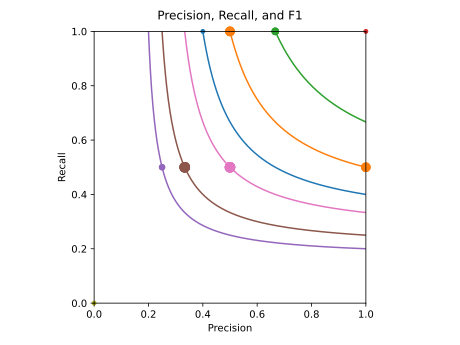
\includegraphics[width=0.6\textwidth]{images/scatter_precision_recall_f1.pdf}
\caption{F1 score isoquants showing how different combinations of precision and recall can yield the same F1 score. Each curve represents a constant F1 value.}
\label{fig:f1-isoquants}
\end{figure}

In \cref{fig:f1-isoquants}, it is clear that the green dot is better than the purple dot because it has both a better precision and recall score. Again, it's not obvious which orange dot is better. The F1 score takes a stance by saying they are tied. Notice the curvature of the F1 isoquants as well. The convexity of the region above the curve means that averages are preferred to extremes, roughly. Any dot on the line segment connecting the two orange dots would have a higher F1 score and thus correspond to a better model.


\subsubsection{Precision--Recall (PR) Curves}

The PR curve plots \emph{precision} (y-axis) against \emph{recall} (x-axis) as vary a model's decision threshold. Let the \emph{prevalence} be $\pi = \Pr(Y=1)$. Useful facts:
\begin{itemize}
\item At extreme low thresholds (label everything positive), recall $=1$ and precision $=\pi$.
\item A random classifier that ignores $X$ yields $\mathbb{E}[\text{precision at any recall}]=\pi$; its PR curve is a flat horizontal line at $y=\pi$.
\item Better-than-random models lie above the baseline for a wide range of recalls; higher \emph{area under the PR curve} (AUPRC) is better.
\item Threshold trade-off: increasing the threshold typically increases precision (fewer predicted positives) and decreases recall; lowering it does the opposite. PR is often more informative than ROC under class imbalance because the baseline and AUPRC depend on $\pi$.
\end{itemize}

\begin{figure}[H]
\centering
% requires \usepackage{tikz}
\begin{tikzpicture}[x=6cm,y=6cm]
  \def\prev{0.30} % prevalence \pi (shown for illustration)
  % axes
  \draw[->] (0,0) -- (1.05,0) node[below] {Recall};
  \draw[->] (0,0) -- (0,1.05) node[left] {Precision};
  % ticks
  \foreach \x/\lbl in {0/0,0.5/0.5,1/1} {
    \draw (\x,0) -- (\x,-0.015) node[below] {\small \lbl};
  }
  \foreach \y/\lbl in {0/0,0.5/0.5,1/1} {
    \draw (0,\y) -- (-0.015,\y) node[left] {\small \lbl};
  }
  % random baseline at prevalence
  \draw[dashed] (0,\prev) -- (1,\prev);
  \node[right] at (1,\prev) {\small random baseline $=\pi$};
  % an illustrative PR curve (monotonically decreasing in practice)
  \draw[thick]
    plot[smooth] coordinates {
      (0.05,0.95) (0.15,0.90) (0.30,0.80) (0.50,0.62)
      (0.70,0.50) (0.85,0.36) (1.00,\prev)
    };
  % threshold trade-off annotations
  \fill (0.30,0.80) circle (0.0075) node[above left] {\scriptsize high threshold};
  \fill (0.85,0.36) circle (0.0075) node[below right] {\scriptsize low threshold};

\end{tikzpicture}
\caption{Precision--Recall (PR) curve with random-classifier baseline at the prevalence $\pi$. Lower thresholds move rightward (higher recall) and typically downward (lower precision), illustrating the trade-off.}
\label{fig:pr-curve}
\end{figure}



\subsection{Experience and Training}

Our computer programs learn from \textit{experience} by being \textit{trained} on data. The training process involves adjusting model parameters to improve performance on the chosen metric.

In reality, the bail prediction problem faces a prohibitive missing data problem. In practice, we only observe outcomes for defendants who were actually released. We never learn what would have happened to those who were detained, so we can never obtain counts for true or false positives. Clever researchers work around this limitation. \cite{kleinberg2018human} exploits a natural experiment: comparing decisions by judges with different release tendencies to infer what might have happened in the counterfactual cases.

Moreover, our labels themselves are often proxies for what we really care about. When predicting ``crime,'' we typically observe arrests or convictions—not actual criminal behavior. Many crimes go unreported or unsolved. This means our training data, while probably useful, is not perfect.

As the statistician George Box famously said, ``All models are wrong, but some are useful.'' The question isn't whether our data perfectly captures reality (it doesn't), but whether our models can still provide valuable insights despite these limitations. In many cases, even imperfect predictions can improve upon human decision-making—as long as we remain clear-eyed about what our models can and cannot tell us. Finally, remember that your models cannot necessarily tell you anything without appropriate problem-specific knowledge. \cite{kuhn2013applied} discusses this in the introduction (Section 1.2).

\subsection{Summary}

We introduced the concept of a learning problem. This requires a performance measure and a way to use data (experience) to improve model performance. Prediction tasks are focal and when we have labeled data, we can use supervised learning techniques. We showed that the choice of a performance measure is (1) ambiguous because there are usually multiple plausible candidates and (2) substantive as it can lead you to prefer one model over the other. This highlights the \textbf{role of the researcher} in possessing problem-specific knowledge and technical knowledge. There is not generally a one-to-one mapping from learning tasks to particular models. The no free lunch theorems of \cite{wolpert1996lack} show that for any two learning algorithms, one won't outperform the other in all contexts, aligning with the agnostic approach to machine learning methods advocated by \cite{grimmer2021machine}. This places the burden on the researcher to understand and explore different models.